%%%%%%%%%%%%%%%%%%%%%%%%%%%%%%%%%%%%%%%%%%%%%%%%%%%%%%%%%%%%%%%%%%
%%%%%%%% CPSC 66 FALL 2023  REPORT %%%%%%%%%%%%%%%%%%%%%%%%
%%%%%%%% This template is modified from ICML 2014 %%%%%%%%%%%%%%%%
%%%%%%%%%%%%%%%%%%%%%%%%%%%%%%%%%%%%%%%%%%%%%%%%%%%%%%%%%%%%%%%%%%

\documentclass{article}

%include any external packages here.  This is similar to loading a
%library in python or C++
\usepackage{clrscode3e} % For codebox
\usepackage{enumitem} % For bullet points

% use Times
\usepackage{times}
% For figures
\usepackage{graphicx}
\usepackage{subfigure}

% For citations
\usepackage{natbib}

% For algorithms and pseudocode
\usepackage{algorithm}
\usepackage{algorithmic}

%Adds hyperlinks to your citations automatically
\usepackage{hyperref}

% Packages hyperref and algorithmic misbehave sometimes.  We can fix
% this with the following command.
\newcommand{\theHalgorithm}{\arabic{algorithm}}

\usepackage[accepted]{icml2014}


% If your title is long (below), use this command to also provide
% short version.  This will go on the top of every page
\icmltitlerunning{Final Report}

\begin{document}

\twocolumn[ %use two column if you need a text to span across the whole page
\icmltitle{ CPSC 66 Final Report: \\ % \\ force a new line
Efficiently and Accurately Classifying Major League Baseball Pitches }

\icmlauthor{Zachary Potthoff}{zpottho1@swarthmore.edu}
\icmlauthor{Alex Rimerman}{arimerm1@swarthmore.edu}

\vskip 0.3in
]

\begin{abstract}
  As baseball grows more technologically advanced, more data 
  is produced every day in all aspects of the game. In this paper, we will focus on MLB's pitch 
  tracking data and how it can be used to classify pitches. It is common to go to a Major 
  League Baseball game, watch a pitch be thrown, and see the pitch type appear on the scoreboard 
  seemingly instantaneously. So, we investigated models to replicate this process and do so in an 
  efficient and accurate manner, just like what is seen at the professional level. We found success 
  in classifying a given pitch at an accuracy rate greater than 90\% and in under 1 second of 
  runtime per pitch. Additionally, some pitches are quite similar to one another, namely the slider and cutter, 
  but are not always consistent with how humans name them. As an extension of our classification, 
  we look into potential human misclassifications of pitch type based on what our algorithm 
  interprets them to be based on their pitch properties, where we do find some differences. We finally 
  take a brief look at the complexity of clustering similarities in pitches and how that is not 
  a simple calculation like one may think. 
\end{abstract}

\section{Introduction}
\label{introduction}

Simply due to the nature of the game, baseball is one of the most statistically-based 
sports one can play. Hitters aim to improve statistics such as batting average or on base 
percentage (OBP), while pitchers want to lower their earned run average (ERA) or walks hits per inning 
pitch (WHIP). However, there is no such thing as one-size-fits-all when it comes to baseball. 
There are successful pitchers who throw hard just as there are unsuccessful pitchers who throw 
hard, yet without seeing both in a game even veteran scouts can struggle to tell the difference. 
In a similar manner, there are pitchers with a good curveball and a bad curveball. Yet, in 
stark contrast to a good and bad pitcher, just about any baseball fan can tell that 
it's a curveball nonetheless.

So, there must be something going on with our ability as humans to identify what pitch is 
being thrown, even if two pitchers throw this same pitch quite differently. With baseball's 
recent advancements in pitch-tracking technology, there is a plethora of advanced metrics out 
there about pitches being thrown in Major League Baseball games. By utilizing this data, we 
attempt to build a model that can correctly classify a pitch in an efficient manner. 
We know that it is possible as it is seen on a daily occurence at Major League games, but 
it also assists in investigating what is going on in the human brain that can properly 
identify a pitch.

We also know that as humans, pitchers sometimes call their pitches different from 
what others would call it. Because of this, we use our algorithm to determine if there 
are any large misconceptions on what a pitch actually is versus what it is called. Lastly, 
as an extension in a different area, we begin to take a look at the complex problem of 
what makes up a good pitcher. We attempt to propely group together similar pitch types, 
investigating if their are commonalities between elite-level pitchers and lower-level ones. 

For this project, we set forth with the goal of creating a pitch classifier that labels 
pitches with $90\%$ accuracy and 1 second of runtime per pitch. This seemed like a reasonable goal 
as it nicely blends both accuracy and efficiency to a sufficient level for a four week 
project. We note that we assume the model to have access to Major League Baseball's 
pitch tracking technology to input our data.

\section{Methods}
\label{methods}

\subsection{Getting the Data}
\label{data}

To collect our data, we wanted to scrape every pitch thrown from the 2023 MLB season. As 
a popular sport for machine learning and data analytics, there are already tools to do this. 
So, we used the open source code from the pybaseball library \cite{pybaseball}.
Utilizing the steps they provide, we were then able to scrape each pitch and its analytical 
data from Baseball Savant, one of the major collectors of baseball data. 

Once pybaseball scraped the pitch data as a Pandas dataframe, we 
then filtered it to only include features we felt were important to 
classifying pitches as well as eliminating any pitches that were missing 
data. For our initial attempt, we decided to include pitch velocity in miles per 
hour, pitch spin rate in rotations per minute, horizontal pitch movement in feet, and 
vertical movement in feet as our features. Because we are doing supervised learning, we 
pull pitch type as a label. As a way of starting our analysis small 
and working in gradual steps, we scrape a smaller data set only consisting of pitches thrown 
in the 2023 World Series to work on first as well as a larger data set that includes all pitches 
thrown in the 2023 MLB season as a final target. 

\subsection{Classifying Pitches}
\label{classify}

Upon filtering our data properly, we decided on a proper model to classify pitches. We 
first considered the properties of our data to decide what the best model could be. Most 
glaringly, we noted that given the drastic differences in units for pitches (e.g. 
pitch spin rate is on the order of thousands but pitch movement is on the order ones), 
we either needed to normalize our data or use a model where units are irrelevant. 
Additionally, we hypothesized that not all features are of equal importance in 
determining pitch type. For example, pitch velocity seems much more important than 
spin rate as a pitch that is 95 mph is much more likely to be a fastball than a curveball, 
yet for a pitch that spins at 2500 rpms, that choice is not obvious without more data. 

From these two observations alone, the properties of the data appeared to line up 
quite well with the advantages presented by a decision tree. To reduce error further, 
we also set the algorithm up to utilize a random forest of decision trees. By doing 
so, in theory we were able to reduce error as we increase the complexity, being careful 
not to overfit. After fitting our data to this random forest, we were able to check 
the effectiveness of it by calculating the accuracy rate of the model. The algorithm 
is as follows:

\textbf{\underline{Input}}
\begin{itemize}[noitemsep]
  \item $df$: a Pandas dataframe of pitch metrics

  \item $pitcherHand$: a char data type indicating if the model is to be built for right-handed 
  or left-handed pitchers
\end{itemize}

\textbf{\underline{Output}}

\begin{itemize}[noitemsep]
  \item Accuracy and confusion matrix of pitch classifications
\end{itemize}

\begin{codebox}
  \Procname{\proc{pitchClassifier}($df$, $pitcherHand$)}
  \li filter out missing data in $df$
  \li \If $pitcherHand$ is 'R': \Then
  \li filter to use right-handed pitchers
  \End
  \li \Else: \Then
  \li filter to use left-handed pitchers
  \End
  \li filter to pitches in consideration for classifying
  \li set pitch type to be the target label
  \li split data into train and test data
  \li train random forest
  \li test random forest and output accuracy
  \li build and output confusion matrix
\end{codebox}

With our project, we initially set forth a goal of making our model $90\%$ accurate and have the 
ability to output a classification of a given pitch within 1 second. This seemed reasonable 
for a four-week timeline as we did not have time for a particularly advanced model, but could 
still find one that models the situation reasonably well. 

Additionally, we worked methodically to progress through the project by starting with a small "toy" 
dataset (e.g. only classifying fastballs and curveballs in the World Series) before moving 
towards larger, more complex datasets. We will not acknowledge each small and fine detail 
of going through the various datasets as that would be excessive and unnecessary; these details 
can be seen in our code if desired. Rather, we will focus on key experiments and results.

\subsection{Evaluating Pitch Differences}
\label{pitchdiff}

Foreshadowing some of our results, after running our initial tests on pitch classification, 
we noticed that issues arise with pitch misclassifications. Most of these occurred on pitches 
that humans could possibly have a hard time distinguishing as well. From this result, we were 
prompted to look into potential factors that we missed that were actually quite important in 
classifying pitches. To do this, we began by looking at one of the most prevalent pairs 
of mislabeled pitches: cutters and sliders.

Using these results, we then began to get a sense of if the new features greatly assisted 
in pitch classification, allowing us to improve our model. This is discussed more in 
section~\ref{results}.

\subsection{Grouping Similar Pitches}
\label{pitchsim}

Lastly, we decided to attempt an extension of grouping similar pitches. This was done with the 
intent of being able to group pitchers who throw comparable pitch arsenals. Then, if successful, 
we could look at what pitchers cluster together and if their stats are comparable, possibly 
helping us draw conclusions about what makes for a successful pitcher. In order to do 
this, we attempt to use a normalized KNN to find the nearest neighbors of an arbitrary 
pitch. Here is our algorithm:

\textbf{\underline{Input}}
\begin{itemize}[noitemsep]
  \vspace{-.1in}
  \item $df$: a Pandas dataframe of pitch metrics
  \item $pitcherHand$: a char data type indicating if the model is to be built for right-handed 
  or left-handed pitchers
\end{itemize}

\vspace{-.15in}

\textbf{\underline{Output}}
\begin{itemize}[noitemsep]
  \vspace{-.1in}
  \item 5 most similar pitches to a given pitch
\end{itemize}

\vspace{-.25in}

\begin{codebox}
  \Procname{\proc{SimilarPitches}($df$, $pitcherHand$)}
  \li filter out missing data in $df$
  \li \If $pitcherHand$ is 'R': \Then
  \li filter to use right-handed pitchers
  \End
  \li \Else: \Then
  \li filter to use left-handed pitchers
  \End
  \li establish label as player name
  \li normalize the data
  \li split data into train and test sets
  \li train KNN on the data
  \li output 5 most similar pitches for each test pitch
\end{codebox}

\section{Experimentation}
\label{results}

In order to achieve our desired results of $90\%$ accuracy in under 1 second
per pitch, we worked sequentially by starting simple and expanding to more complex 
data and methods. 

Please note that for our results, we utilize confusion matrices with abbreviations 
for pitch types. Here is the \hyperref[key]{key}.

\subsection{Pitch Classifier}

\subsubsection{Experiments \& Results}
Following from the methods section,
we started with only distinguishing between fastball, curveball, and changeup. To do this,
we simply filtered our data set to only include these pitch types. From there we split
our data into train and test, and fit our Random Forest model. Then we tested the test set
and produced the following confusion matrix:

\vspace{-.1in}

\begin{center}
  \begin{figure} [!ht]
    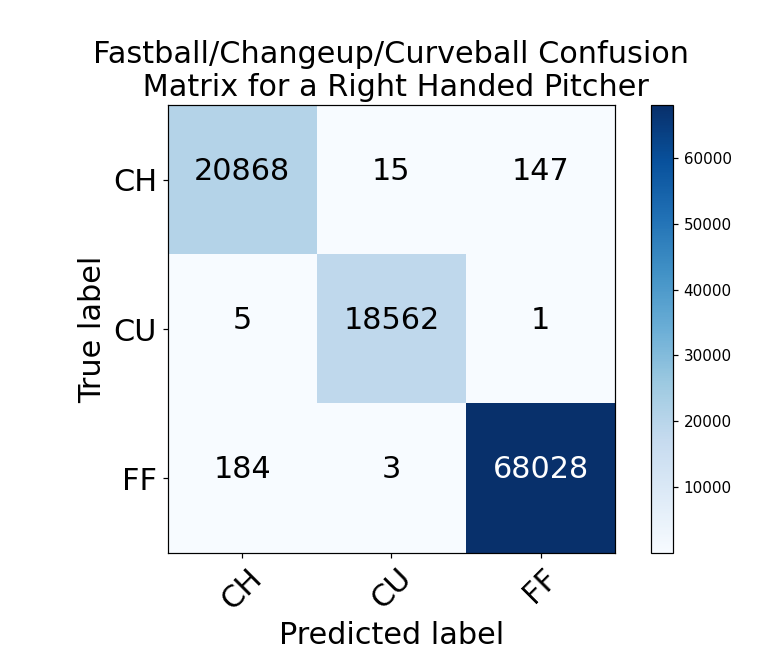
\includegraphics[scale = .22]{FCCR-R.png}
    \caption{An initial confusion matrix}
    \vspace{-.3in}
  \end{figure}
\end{center}

In this version of our algorithm, the model predicts pitches with $99.7\%$ accuracy.
Based on this, we determined that moving forward and adding more pitch types was an 
appropriate next step. From here, we continued with the same
parameters as before, but now with the entire 2023 season of pitches to get a baseline of 
how well our model behaves. This output can be seen
in the next two confusion matrices, one for right-handed pitchers, and one for left-handed
pitchers:

\begin{center}
  \begin{figure} [h!]
    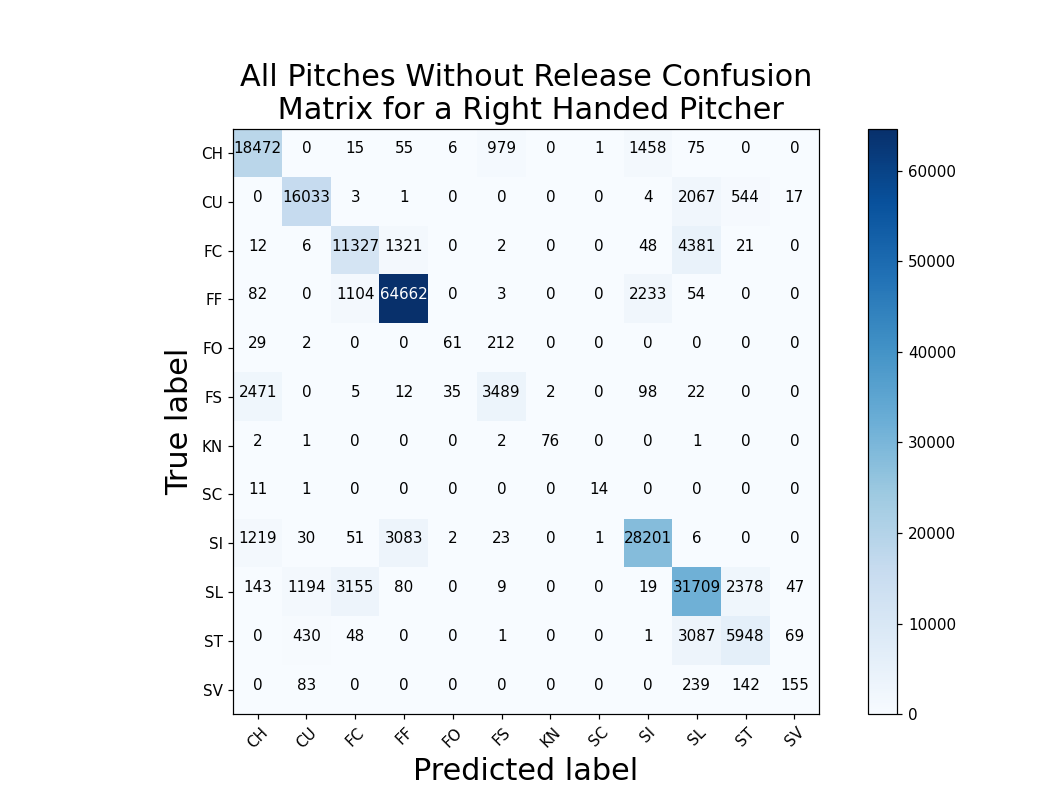
\includegraphics[scale = .26]{FNR-R.png}
    \caption{Second stage confusion matrix (Right-Handed Pitcher)}
  \end{figure}
  \begin{figure} [h!]
    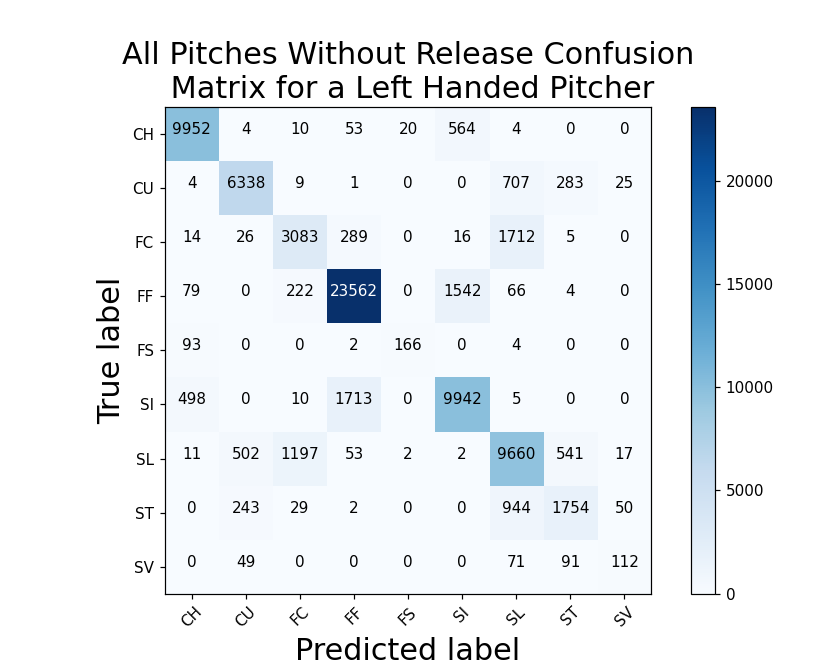
\includegraphics[scale = .31]{FNR-L.png}
    \caption{Second stage confusion matrix (Left-Handed Pitcher)}
  \end{figure}
\end{center}

This data did not perform as well as the prior, outputting an accuracy of $84.5\%$
for both right-handed and left-handed pitchers. Thus, we determined that our data or algorithm must not
be adequate enough to complete our task. There are certain pitches that blend too closely
together for our model to handle, prompting us to consider the potential causes of this misclassification.

\subsubsection{Initial Discussion}

If we look at our results, we see a large disparity when we increase from only classifying 
three pitches to then trying to classify all pitches. This is not a surprising result, and 
was actually done with intention. In creating our model, we wanted to start with attempting 
to classify three very different pitches in terms of their properties. Fastballs, curveballs, 
and changeups are about as distinct as three pitches could be. This seemed to be a nice 
starting point because it allowed us to get a sense of if we chose a proper model. Given that the model 
performed with $99.7\%$ accuracy and a negligible amount of confusion (mostly all between fastballs 
and changeups), we felt fairly confident in our choice of a Random Forest for modeling this problem. 
Additionally, of the confusions, the amount of fastballs and changeups that were misidentified were 
not a concern because we did not expect a perfect model and fastballs and changeups are not completely 
different pitches in some cases.

As we moved into classifying more pitches, however, we started to see a drop off in accuracy, culminated 
by the result given above of $84.5\%$ accuracy for all pitches thrown across the 2023 MLB season. 
With more pitches in consideration, their properties begin to fuse together as there is only so 
much movement, velocity, and spin that is humanly possible. So, in an unsurprising way, we see the 
accuracy suffer as similar pitches get confused with one another as seen in the confusion matrix. 
For example, sliders and cutters as well as sweepers and sliders often get mixed up with one another. 
As most baseball players could say, this makes sense as they are extremely comparable pitches. From 
this, we figured that we needed another feature to help the decision trees narrow their search spaces 
to more accurately classify which pitch is which.

One piece of information that is commonly used to decipher a pitcher's arsenal is their arm 
angle and release point. Considering that release point is a product of arm angle, we figured 
there would be benefit for our algorithm to work with release point. Additionally, we 
hypothesize that there is more information to be gained through release point. For example, 
a pitcher who releases the ball at shoulder height is more likely to be throwing a 
sweeper than a slider, whereas a pitcher who releases the ball above his head is more likely 
to be throwing a slider than a sweeper. We do not cite any material here because this is simply 
from knowing the physical requirements to throw both pitches. So, we then ran similar experiments 
while including vertical release height in feet and horizontal release distance in feet as features.

\subsubsection{Release Point Experiments}

To start our implementation of the new features, we chose two of the most commonly confused pitches by the model.
When looking specifically at cutters and sliders, we see a lot of mislabeling between 
the two pitches. For the baseball community, this makes intuitive sense because they are very similarly moving pitches. 
So, if the predictions are more accurate with release data by a reasonable margin, we know it is better 
and can look to apply the additional features to larger data. This can be seen in the following images:

\begin{center}
  \begin{figure} [h!]
    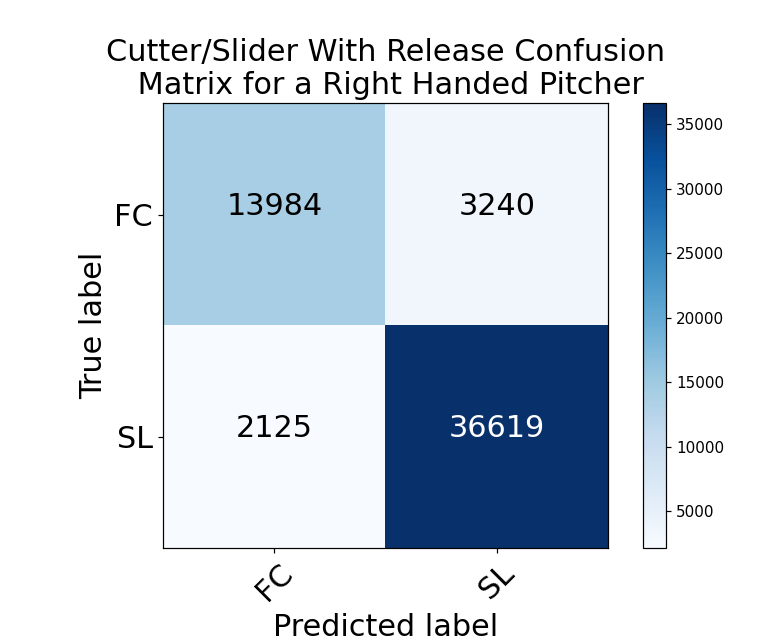
\includegraphics[scale = .14]{CSR-R.png} 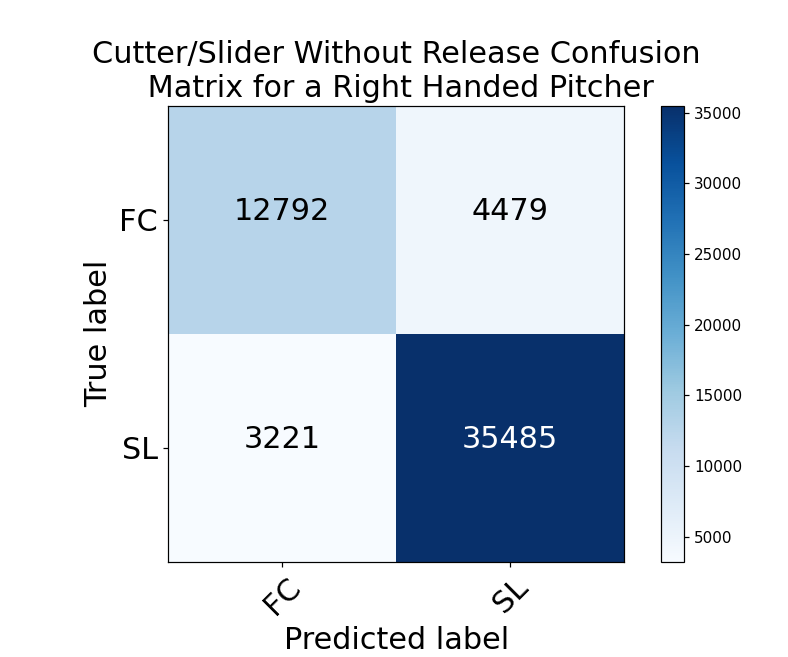
\includegraphics[scale = .14]{CSNR-R.png}
    \caption{A comparison of cutter and slider confusion matrices}
  \end{figure}
\end{center}

We can see here how much better the model with release point data (left) performs compared to without
release point data (right). The with release model distingued between the two pitch types with $90.4\%$
accuracy, whereas the model without release point data performed at $86.2\%$ accuracy. This is a very 
significant increase given a very big sample size. Thus, we tried to build the full model
using this new data. This confusion matrix can be seen here:

\begin{center}
  \begin{figure} [h!]
    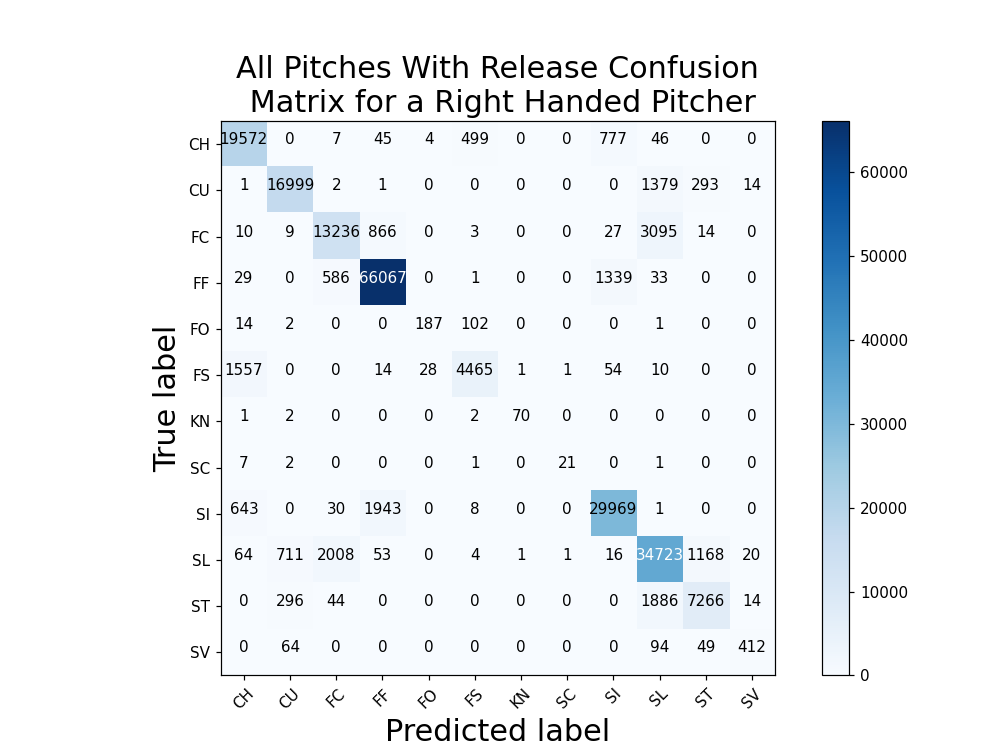
\includegraphics[scale = .23]{FR-R.png}
    \caption{Final model confusion matrix}
  \end{figure}
\end{center}

We see an increase in accuracy when using the release features. Our model improved to prediction
with $90.4\%$ accuracy for right-handed pitchers as opposed to the $84.5\%$ from before. While the confusion matrix is not included
here, we saw an even bigger jump in accuracy for left-handed pitchers when including
release features, improving from $84.5\%$ to $93.2\%$.

\subsubsection{Further Discussion}

Looking at these new results with the additional features, we can see a significant increase in accuracy.
This increase shows that the addition of the release point data for each pitch was able to solve our issue
from before. We are now able to predict pitch types with over $90\%$ accuracy. In conjunction with this 
higher accuracy, we see an improvement in the confusion of similar pitches that presented issues earlier. 
For example, in our initial model, sweepers were mislabeled as sliders approximately $32\%$ of the time in contrast to 
the new model, which only was confused in this fashion about $20\%$ of the time. 

Initially, we were fairly
surprised by how drastic of an increase was seen with this addition of pitch release data. We thought that velocity, movement, and
spin would be enough to distinguish between all of the pitches. However, digging deeper, we ultimately
realized that this increase makes sense because of the implications of a pitchers release. A pitcher's
arsenal of pitches tends to be a direct result of how and where they release the ball. Certain releases
are more optimal for some pitches but not others. Given that we are utilizing data from Major League Baseball, it is no
surprise that most of the pitchers would be taking advantage of this, allowing for more similarities in our data.

Another feature that could have been very beneficial for pitch classification is the idea of spin direction.
This feature is utilized
to determine on what axis a pitch spins on. It uses the times on a clock to observe in what direction the 
ball is spinning. For example, a 12:00 spin direction would mean perfect back spin, and 6:00 would be perfect
top spin. However, a number like 1:00 would mean that a right-handed pitcher is back spinning the baseball
but the angle the ball is released is 30 degrees from North. Typically, spin direction along with movement
is what distinguishes pitches like a curveball or slider comapred to a slurve or a sweeper.
Unfortunately, we were not able to use this because we could not find a way to properly quantify 
the idea of how a clock is scaled in a circular nature (e.g. 12:30 and 1:00 are only 30 minutes away) in 
a usable way for a decision tree. We expect that if we were able to include this data, our model 
would improve even more.

\subsection{Similar Pitch Identification \& Discussion}

An extension of our project that we tried to implement within the last week of lab was a model that given a
pitch would output the 5 most similar pitches also thrown in the 2023 season. Using the algorithm that was laid out in
pseudocode in~\ref{pitchsim}, here is an example of four outputs:

\begin{center}
  \begin{figure} [h!]
    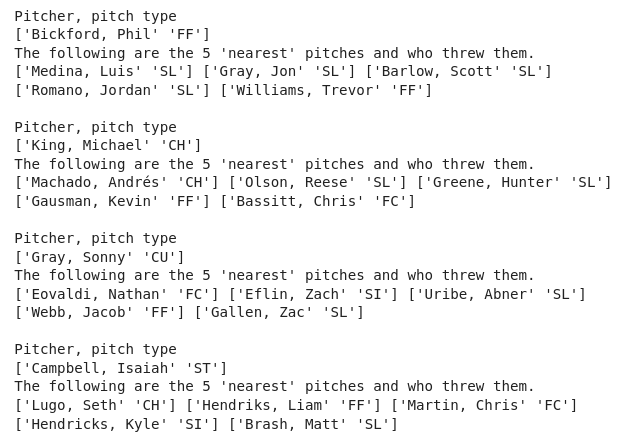
\includegraphics[scale = .35]{GroupSimPitch.png}
    \caption{Output of similar pitch algorithm}
  \end{figure}
\end{center}

In theory, we expect pitches to be most similar to other pitches of the same label. We clearly see here that 
very different pitch types get listed as neighbors of one another by KNN (e.g. Phil Bickford's fastball is 
similar to Luis Medina's slider according to the model). Due to time constraints, we were unable to look 
further into this problem. However, the fact that this problem arose offers some insight into the complexity 
of this task as we see that it is not linear in nature. We hope to continue our investigation of this in 
the future.

\section{Ethics \& Social Implications}
\label{ethics}
We acknowledge that for this specific project, there are minimal impacts on the baseball community. This 
was expected going into the project as it was only a four week project. Major League Baseball has similar 
technology which was part of the inspiration of our project. As the best baseball league in the world, 
the MLB has a neural network model to classify pitches in real time at their games \cite{Sharpe_Schwartz_2020}. 
As such, it is not realistic to think that anyone would choose to use our model over the MLB's and some 
other models that are out there. However, for the purpose of this discussion, we will consider the ethical 
and social implications as if we continue to improve our model and project to a level that is the leading 
algorithm used in pitch classification.

To begin, we will first consider the key stakeholders in a project like this. These stakeholders include 
Major League Baseball organizations and everyone in them, baseball fans, and baseball technology companies. 
If we look within the organizations, we see a wide variety of users. This includes coaches and players who are 
trying to elevate their team's performace as well as scouting departments who want to analyze potential 
prospects. By providing such a model for general use, this puts organizations on a level playing field. It 
is not difficult to imagine a scenario if this technology does not exist publicly where some organizations gain a 
serious step ahead of others by privately developing a similar technology. In addition, from a fan's 
perspective, having such a technology for general use can enhance the viewing experience by adding 
additional context to the game. There are no obvious drawbacks to this and can generally be considered a 
positive for all fans. 

As far as group and power dynamics, we will focus more so on major technology companies as stakeholders 
as it is most applicable in this business. If we consider the idea of a public versus private code release,
we see that the power dynamics change. If this technology were to be public, the power dynamics seem fairly 
mitigated because it creates a more equal opportunity for all companies. Moreover, it empowers baseball research 
and development to advance the game at a greater rate than ever before. On the contrary, if this code 
were to be privately sourced and sold as a product, power dynamics would play a very heavy role. For example, 
this potentially leads to the possibility of monopolization of baseball technology because the companies 
with more buying power are able to purchase the product, whereas it might be overpriced for small businesses. 
This severely impairs research and development for the baseball community.

From the hypothetical perspective we are taking here, it is easy to see that the overall community 
would benefit more from a free, public release of top quality pitch classifying technology. However, 
the realistic economic perspective says that this is quite unlikely as Major League Baseball and baseball 
technology are massive markets. This would likely lead to extremely competitive offers, some that many 
may consider irrefusable. As with all new and improving technology in other areas, economically beneficial 
goals tend to dominate the market.

\section{Conclusions}
\label{conclusion}

Overall, we deemed that our project was very succesful given the time aspect. Our original goal of this 
project were to see if we could replicate Major League Baseball's pitch detection system in a more simple,
but efficient way. Specifically, these goals included $90\%$ accuracy in 1 second per pitch. We were able to 
build our model for this pitch classification quite quickly, but we were not meeting our $90\%$ metric. 
From here, we began to brainstorm ideas on how to combat this, deciding on implementing more features 
into our dataset. In order to determine if adding these features was successful, we built a simpler model 
that distinguished between two similar pitch types; we identified this to be a beneficial adjustment 
to the dataset. Moving back into the key objectives, we saw that this adjustment also led to a large 
increase in accuracy without too large of an increase in time complexity, thus satisfying our metric 
goals. 

Upon reaching these goals of accuracy and efficiency, we decided to pursue a different extension of the 
project rather than continuing attempting to improve the classifier. While we do think we could have 
marginally improved the model in the remaining time frame, we concluded that significant improvements 
would require time and complications that were beyond the scope of the remaining week of the project. 
Using this idea of classification, we moved on to attempting to identify similarities between individual 
pitches. Specifically, we wanted to identify a given pitch's five most comparable pitches thrown by 
other pitchers. While the results say that we were not successful in building this model, we gained insight 
into the complexity of this problem. 

From here, we hope to continue the main goal of the project of building an even better 
pitch classification model. We intend to look into further improvements of the model such 
as hyperparameter tuning or even changing the model. One leading idea at the moment is 
building the model as a neural network that becomes more accurate to a level that is 
useful to others. We want this neural network to expand to all pitches, not just the Major 
League level. This would allow us to provide use to all levels of baseball, ranging from 
Little League all the way up to professional. The hope is that we could further baseball 
engagement and development at all stages of the game.

\section*{Acknowledgments}

We would like to thank Professor Benjamin Mitchell in his assistance and advice throughout the course 
of the project. We also would like to thank James LeDoux for his open source contributions with 
pybaseball. We greatly appreciate both of their contributions.


\bibliography{references} 
\nocite{baseballsavant.com}
\bibliographystyle{icml2014}

\newpage

\section*{Pitch Type Key}
\label{key} 
CH: changeup

CU: curveball

FC: cutter

FF: four-seam fastball

FO: forkball

FS: splitter

KN: knuckleball

SC: screwball

SI: sinker

SL: slider

ST: sweeper

SV: slurve


\end{document}


% This document was modified from the file originally made available by
% Pat Langley and Andrea Danyluk for ICML-2K. This version was
% created by Lise Getoor and Tobias Scheffer, it was slightly modified
% from the 2010 version by Thorsten Joachims & Johannes Fuernkranz,
% slightly modified from the 2009 version by Kiri Wagstaff and
% Sam Roweis's 2008 version, which is slightly modified from
% Prasad Tadepalli's 2007 version which is a lightly
% changed version of the previous year's version by Andrew Moore,
% which was in turn edited from those of Kristian Kersting and
% Codrina Lauth. Alex Smola contributed to the algorithmic style files.
